\section{Fokker-Planck equation}
\subsection{Formula derivation}
Now we want to derive the Fokker-Planck equation, that corresponds to the Liouville equation when stochastic contributions are added to the system.\\
We start considering the Ito chain rule neglecting the time dependence of $A(x,t)$ and $B(x,t)$, that is 
\[
dy=y'A(x)dt+y'B(x)dW+\frac{1}{2}y''B^2(x)dt
\]
We now want to propagate the density on the phase space of different copies of the system, and in order to do so we need to count how many copies are present in a volume $\bar{x}$ of the phase space.

\begin{figure}[H]
  \centering
  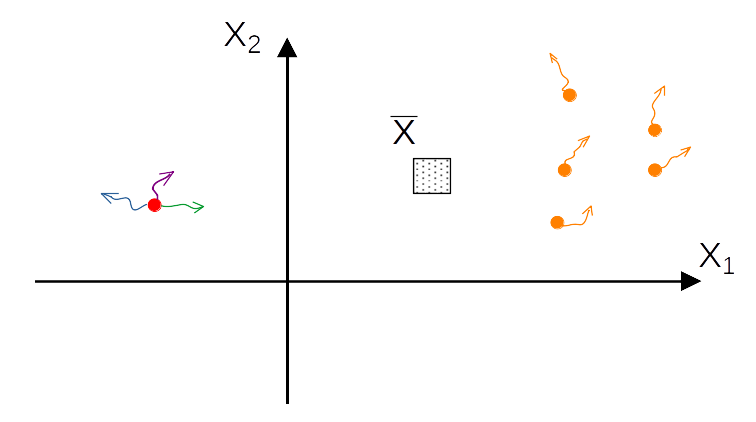
\includegraphics[width=0.8\textwidth]{SDE/Figures/Phase_space_Fokker.png}
  \caption{Two dimensional phase space.\\\hspace{\textwidth}
  Each point represent a specific configuration of the phase space. \\\hspace{\textwidth}
  As the {\color{red} red point} highlights, each point in the phase space can have different evolution due to randomness. On the other hand, we are usually interested in the evolution of an ensemble of many points ({\color{orange} orange points}). $\bar{x}$ represents a volume in the phase space.
  } 
  \label{Fig:Fokker_phase_space}
\end{figure}

Since we are dealing with continuous variables, in order to count the copies, we use the function $y(x)= \delta(x-\bar{x})$, then $y'(x)=\delta'(x-\bar{x}), y''(x)=\delta''(x-\bar{x})$.
Thus for a single trajectory we get
\begin{equation}
dy=\delta'(x-\bar{x})A(x)dt+\delta'(x-\bar{x})B(x)dW+\frac{1}{2}\delta''(x-\bar{x})B^2(x)dt.
\end{equation}
If we consider the double average we have:

\begin{equation}
    \begin{split}
        \langle dy \rangle &=\int dxP(x)\Big\langle\delta'(x-\bar{x})A(x)dt+\delta'(x-\bar{x})B(x)dW+\frac{1}{2}\delta''(x-\bar{x})B^2(x)dt\Big\rangle\\
        & =\int dxP(x)\left[\delta'(x-\bar{x})A(x)+\frac{1}{2}\delta''(x-\bar{x})B^2(x)\right]dt \label{eqn:sub}
    \end{split}
\end{equation}
where the integral represents the average over the phase space, ($P(x)$ is the probability of finding a copy in position $x$), while $\langle \rangle$ is the average among all the copies. The second term vanishes since the noises cancel out taking the average.
Assuming $x$ to be one dimensional and with no boundaries (\emph{i.e.} $x \in (-\infty,+\infty)$) we can compute the two terms in the integral of Eq. \eqref{eqn:sub}. For the first we have
\[
\int dx\left(P(x)A(x)\right)\delta'(x-\bar{x})\underbrace{=}_{\text{by parts}}-\int dx\left(\frac{\partial}{\partial x}P(x)A(x)\right)\delta(x-\bar{x})=-\frac{\partial}{\partial x}P(x)A(x)\bigg|_{x=\bar{x}}
\]
since $P(x)A(x)=0$ at $\pm\infty$. For the second term we have
\begin{equation*}
    \begin{split}
\frac{1}{2}\int dx\left(P(x)B^2(x)\right)\delta''(x-\bar{x})&\underbrace{=}_{\text{by parts}}-\frac{1}{2}\int dx\left(\frac{\partial}{\partial x}P(x)B^2(x)\right)\delta'(x-\bar{x})= \\
&\underbrace{=}_{\text{by parts}}+\frac{1}{2}\int dx \frac{\partial^2}{\partial x^2}\left(P(x)B^2(x)\right)\delta(x-\bar{x})= \\
&\,\,\,\,\,\,=\frac{1}{2}\frac{\partial^2}{\partial x^2}P(x)B^2(x)\bigg|_{x=\bar{x}}.
    \end{split}
\end{equation*}
Thus
\begin{equation}
\langle dy \rangle =\left[-\frac{\partial}{\partial x}\left(P(x,t)A(x)\right)+\frac{1}{2}\frac{\partial^2}{\partial x^2}\left( P(x,t)B^2(x)\right)\right]dt.
\end{equation}
Finally, since $\langle y \rangle =P(\bar{x})$, we get to the Fokker-Planck equation
\begin{equation}
\frac{\partial P}{\partial t}=-\frac{\partial}{\partial x}AP+\frac{1}{2}\frac{\partial^2}{\partial x^2}B^2P
\label{Fokker-Planck equation}
\end{equation}
which is expressed in a compact way neglecting the dependences on $t$ and $x$.




\subsection{Current density J}
If we define the current density $J$ as:
\[
J \equiv AP - \frac{1}{2} \frac{\partial}{\partial x}B^2 P
\]

We can re-write the Fokker-Planck equation (\ref{Fokker-Planck equation}) as a continuity equation:
\begin{equation}
\frac{\partial P}{\partial t} = - \frac{\partial J}{\partial x}.
\label{K-P continuity equation}
\end{equation}

In multiple dimensions:
\[
J_i \equiv A_iP - \frac{1}{2}\sum_j \frac{\partial}{\partial x_j} \left( \sum_k B_{ik}B_{jk} P \right)
\]

and the Fokker-Planck equation becomes:
\begin{equation}
\frac{\partial P}{\partial t} = - \sum_i \frac{\partial J_i}{\partial x_i} \hspace{5mm}\text{with }\hspace{3mm} dx_i = A_idt + \sum_j B_{ij} dW_j.
\label{K-P multidimentonal continuity equation}
\end{equation}


The introduction of $J$ allows us to connect the Fokker-Plank equation to Balance and Detailed Balance. \\
As we know Balance implies that the probability distribution $P$ doesn't change over time. So, using Fokker Plank we can say:
\[
\text{Balance} \hspace{2mm} \implies \hspace{2mm} \frac{\partial P}{\partial t} = 0 \hspace{2mm} \implies \hspace{2mm} \sum_i \frac{\partial J_i}{\partial x_i} = 0.
\]
So, there can be a flux of probability $\partial J_i$ along direction $i$, but the divergence of this flux must be zero. On the other hand, Detailed Balance enforces a stronger condition, that is, there is no flux along any component:
\[
\text{Detailed balance} \hspace{2mm} \implies \hspace{2mm} J_i = 0.
\]

Note that in 1D Detailed Balance and Balance imply the same condition. Indeed we can see that in an infinite domain, assuming Balance implies that $J=const$, but on the other hand $J\propto P$. Since $P(x\xrightarrow{}\pm \infty) = 0$, then $J = 0$. \\

\textbf{Example}:\\
\newline
We can apply the Fokker-Planck equation to a simple example:
\begin{equation*}
    dx = -xdt + dW
\end{equation*}
where we have $A=-x$ and $B=1$, so we obtain:
\begin{equation*}
\begin{split}
    & J=-xP-\frac{1}{2}\frac{\partial P}{\partial x}\\
    & \frac{\partial P}{\partial t} = \frac{\partial}{\partial x}(xP)+\frac{1}{2}\frac{\partial^2}{\partial x^2}P
    \end{split}
\end{equation*}
we can see in Fig. \ref{fok_ex} that the equation above \textit{flatten} $P(x)$, since around the peak the second derivative is negative, hence those points are decreased, while the points in the tails increase due to the positive second derivative. The ultimate result is a flat distribution.

\begin{figure}[H]
  \centering
  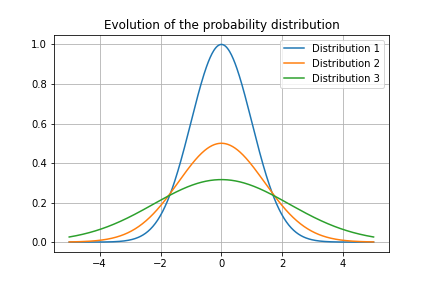
\includegraphics[width=0.7\textwidth]{SDE/Figures/fokker_example.png}
  \caption{Evolution of the distribution following Fokker-Planck. This distribution is just a graphical example, it should not be considered an accurate description of $P(x)$.}
  \label{fok_ex}
\end{figure}
 


\subsection{Example: Sampling from the Canonical Ensemble}
We can use the conditions for balance and detailed balance on $J$ in order to sample from the canonical ensemble.\\
We want to find the coefficient $A$ and $B$ for a given $P(x)$ such that:
\begin{equation*}
    AP - \frac{1}{2}\frac{\partial}{\partial x}\left( B^2 P \right) = 0
\end{equation*}
namely we want to enforce detailed balance.\\
If we fix $B=const$ we can find the correct value for $A$ solving:
\begin{equation*}
    A = \frac{1}{2}\frac{1}{P}\frac{\partial}{\partial x}\left( B^2 P \right)
\end{equation*}
which can be written as:
\begin{equation*}
    A = \frac{B^2}{2}\frac{1}{P}\frac{\partial P}{\partial x} = \frac{B^2}{2}\frac{\partial \log P}{\partial x}
\end{equation*}
where we used the fact that $B$ is constant.\\
We have that $P(x) \propto \exp(-\beta U(x))$, which gives:
\begin{equation*}
    A = -\frac{B^2}{2}\beta \frac{\partial U(x)}{\partial x}
\end{equation*}
Now we have everything we need to write the stochastic differential equation that rules the evolution of $x$. We call $B^2 = 2D$, where $D$ is the \textit{diffusion coefficient}, and we obtain:
\begin{equation}
    dx = -\frac{D}{k_B T}\frac{\partial}{\partial x}U(x)dt + \sqrt{2D}dW
\end{equation}
This equation is called \textit{Overdamped Langevin Equation} and we can see that for large $T$ the dynamic is dominated by the stochastic term.\\

In some particular situations we may also have:
\begin{equation*}
    dx = \sqrt{2D(x)}dW
\end{equation*}
with $A=0$ for simplicity. In this situation we obtain (as before $B^2 = 2D(x)$):
\begin{equation*}
    \frac{\partial D P}{\partial x} = 0
\end{equation*}
which entails that:
\begin{equation*}
    P(x) \propto \frac{1}{D(x)}
\end{equation*}
that can be interpreted as the fact that the particle spends more time in the regions where $D(x)$ is small.